\section[Ordinamento senza confronti]{Algoritmi di ordinamento non basati su confronti}
\subsection{IntegerSort}
È un algoritmo di ordinamento che si basa sulla conoscenza a priori dell'intervallo in cui sono compresi i valori da ordinare.
L'algoritmo conta il numero di occorrenze di ciascun valore presente nell'array 
da ordinare, memorizzando questa informazione in un array temporaneo di dimensione
pari all'intervallo di valori. Il numero di ripetizioni dei valori indica
la posizione del valore immediatamente successivo. 
\begin{itemize}
    \item Si calcolano il valore massimo e il valore minimo, $max(A)$ e $min(A)$
    \item Si prepara un array ausiliario $C$ di dimensione pari all'intervallo 
    di valori con entrate $C[i]$ che rappresentano la frequenza dell'elemento
    $i + min(A)$
    \item Si visita l'array $A$ aumentando l'elemento di $C$ corrispondente.
    \item Si visita l'array $C$ in ordine e si scrivono su $A$ $C[i]$ copie del valore $i + min(A)$ 
\end{itemize}

\subsubsection*{Complessità}
L'algoritmo esegue 3 iterazioni, 2 di lunghezza $n$ per individuare massimo e minimo e per il calcolo delle
occorrenze dei valori, e una di lunghezza $k = (max(A)- min(A) - 1)$.\\
La complessità totale è quindi $O(n+k)$. \\
Conviene utilizzarlo quando il valore di $k$ è $O(n)$.

\begin{figure}[h]
    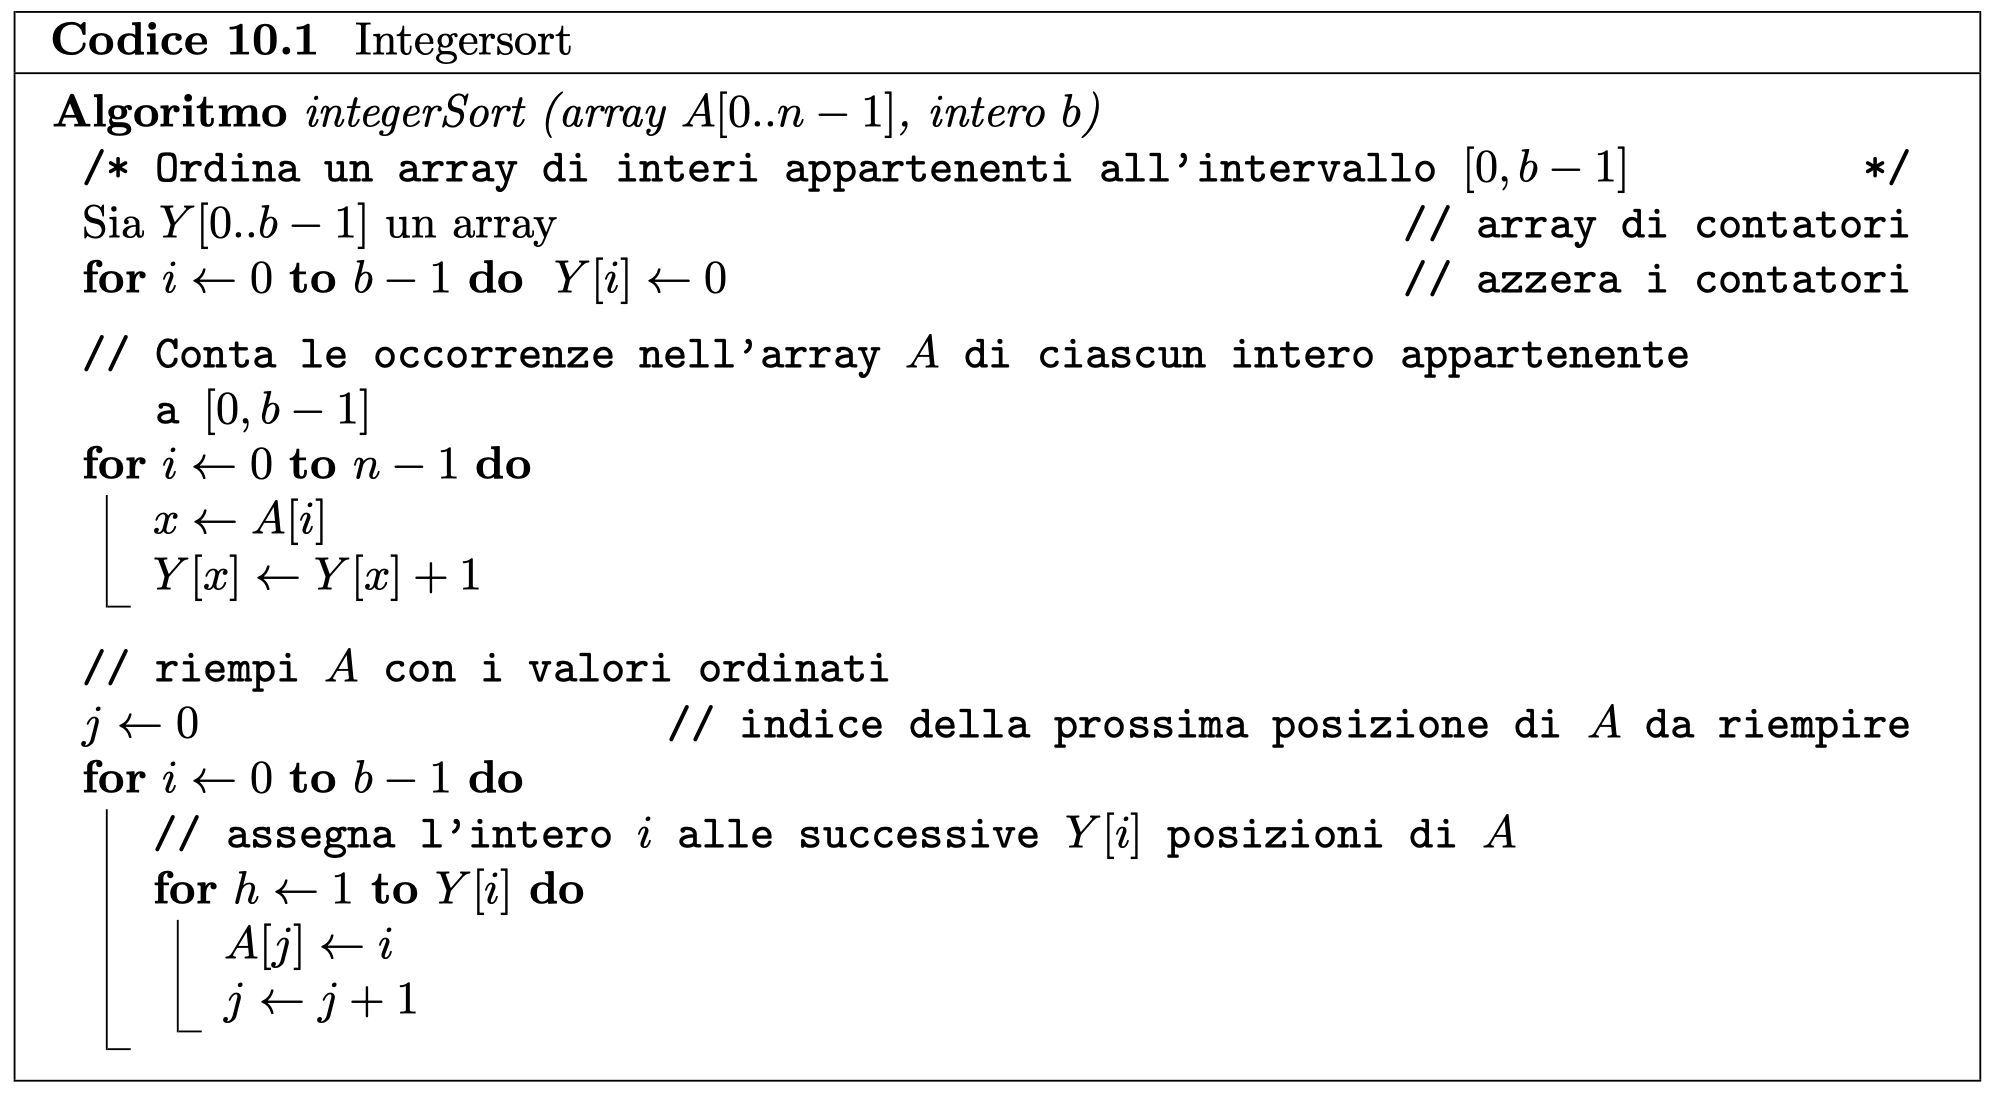
\includegraphics[width=\textwidth]{integerSort.png}
\end{figure}
\clearpage

\subsection{BucketSort}

\begin{wrapfigure}{r}{7cm}
    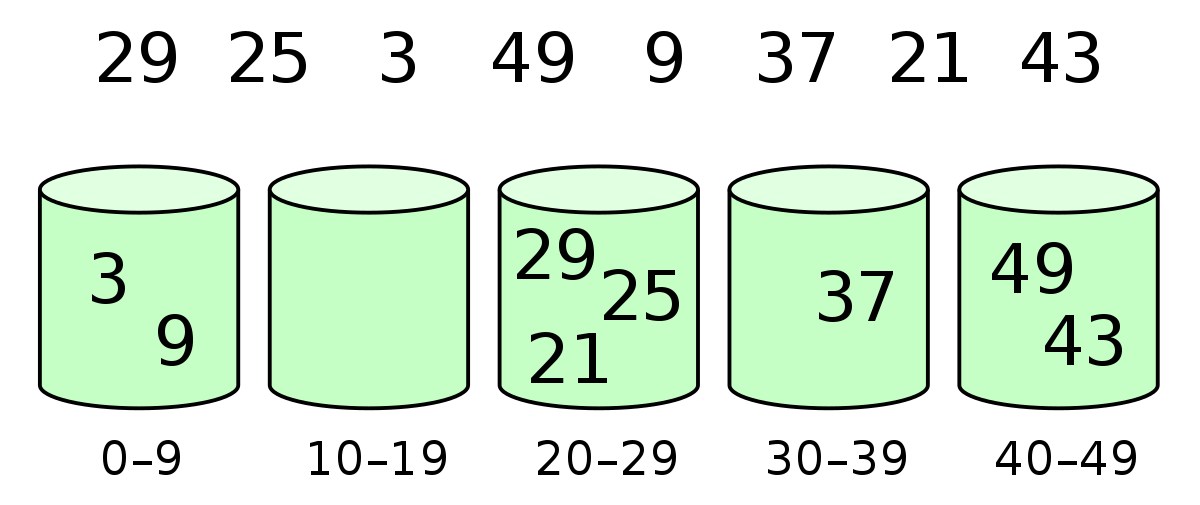
\includegraphics[scale = 0.2]{bucketsort_es.png}
\end{wrapfigure}

È un algoritmo di ordinamento per valori numerici che si assume siano distribuiti
uniformemente in un intervallo $[0,1)$\\
Se $n$ è il numero di elementi da ordinare, l'intervallo $[0,1)$ è diviso in $n$
intervalli di uguale lunghezza, detti \emph{bucket}.
Ciascun valore dell'array è quindi inserito nel bucket a cui appartiene, i valori
all'interno di ogni bucket vengono ordinati e l'algoritmo di conclude con la concatenazione
dei valori contenuti nei bucket.

\subsubsection*{Complessità}
La complessità di \texttt{bucketSort} è $O(n)$ per tutti i cicli, a parte l'ordinamento dei 
singoli bucket. Date le premesse sull'input, utilizzando \texttt{insertionSort}
l'ordinamento di ogni bucket è $\Theta(1)$, quindi la complessità media è
$O(n)$ per tutto l'algoritmo. La complessità complessiva nel caso migliore è 
$O(n+m)$ dove $m$ è il massimo valore nell'array.

\begin{figure}[h]
    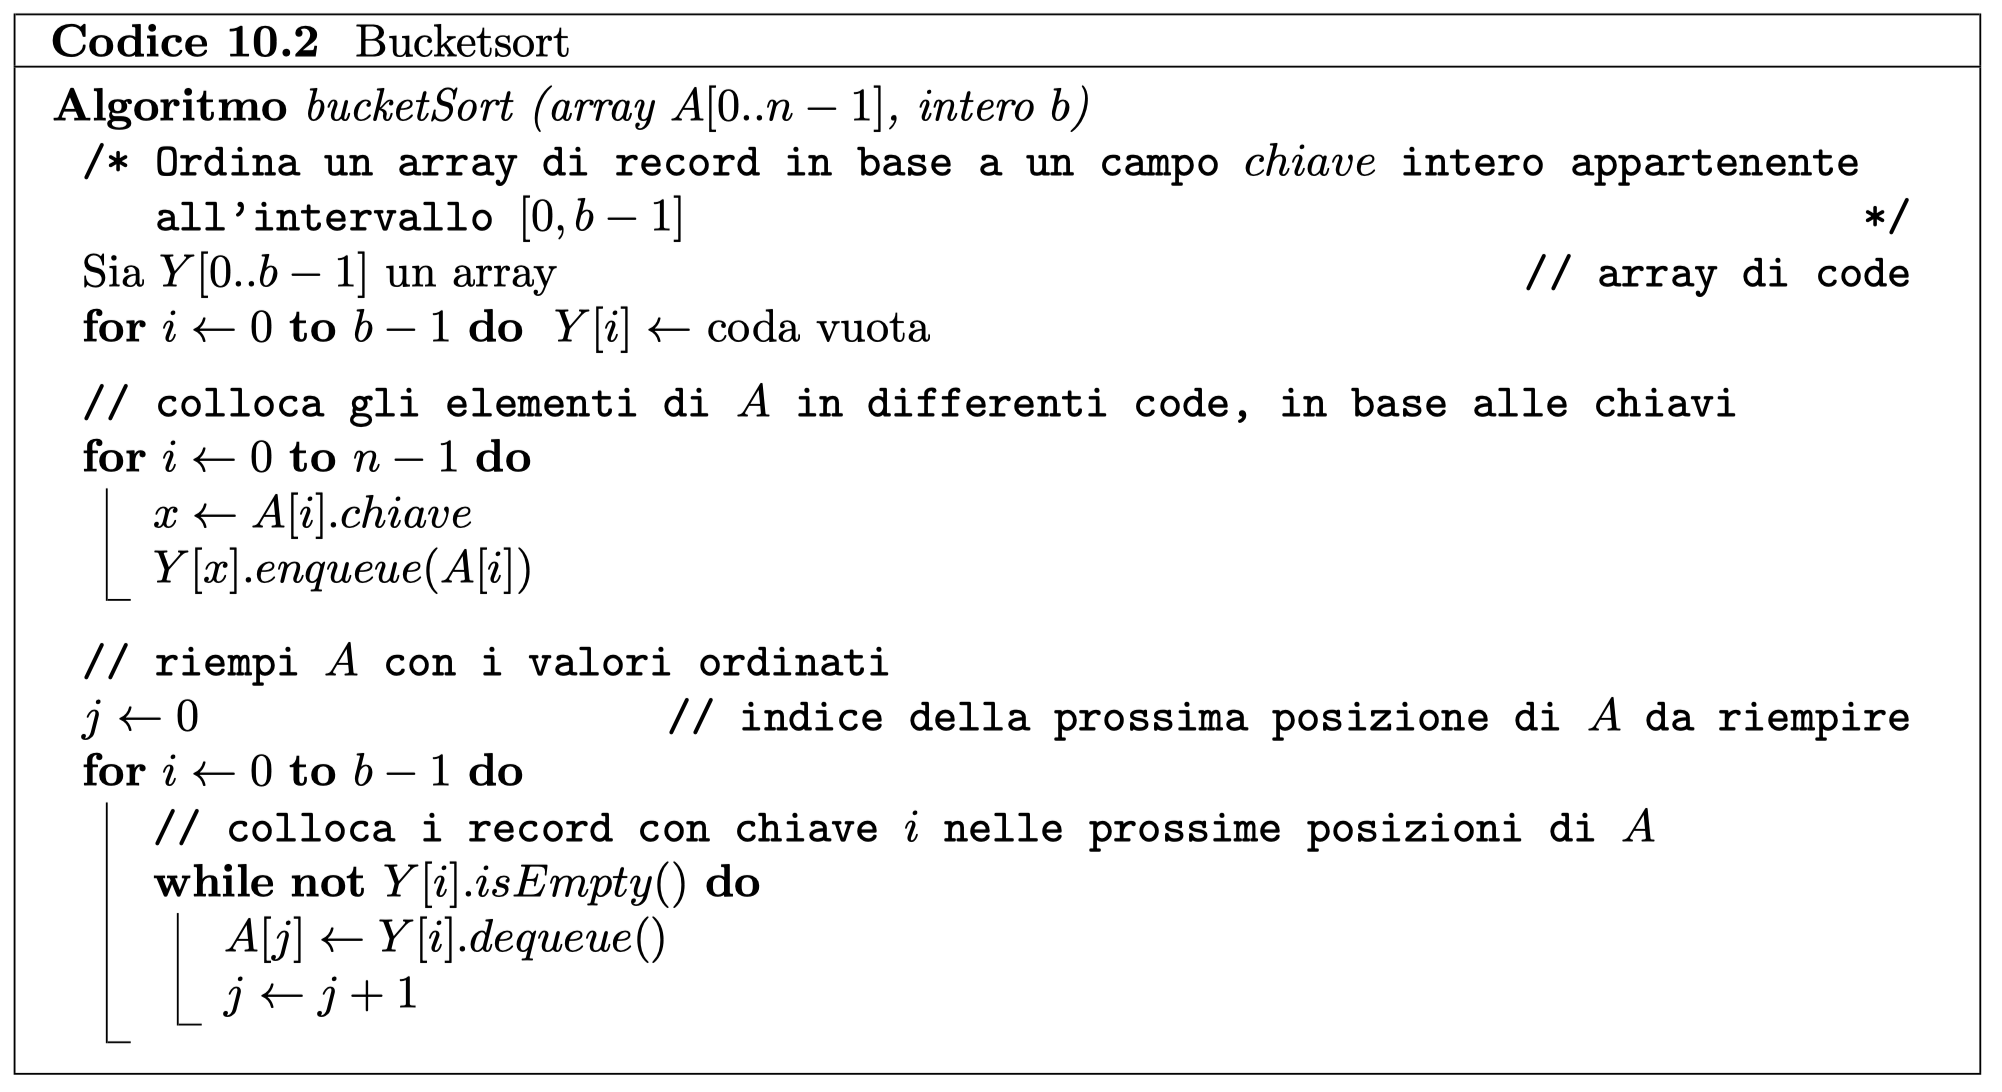
\includegraphics[width=\textwidth]{bucketSort.png}
\end{figure}
\clearpage
\subsection{RadixSort}
È un algoritmo che esegue degli ordinamenti per posizione della cifra, partendo 
dalla cifra meno significativa. Questo affinchè l'algoritmo non si trovi a dovere
operare ricorsivamente su sottoproblemi di dimensione non valutabile a priori.

\begin{wrapfigure}{r}{7cm}
    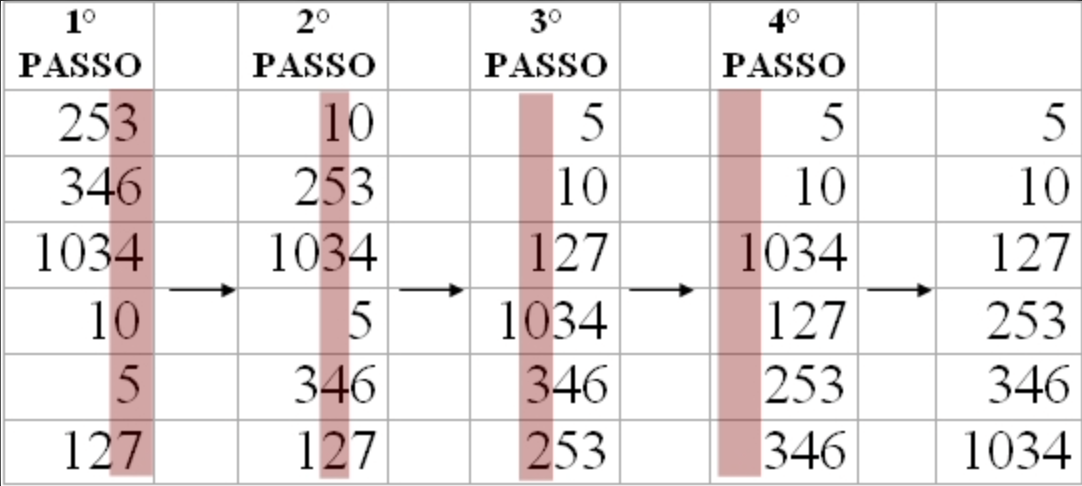
\includegraphics[scale = 0.4]{radixsort_es.png}
\end{wrapfigure}

\subsubsection*{Complessità}
L'algoritmo ha complessità computazionale pari a $O(n\cdot k)$ dove $n$ è 
il numero di elementi da ordinare e $k$ è la media del numero di cifre degli $n$ elementi.
Se $k$ risulta essere minore di $n$ non si ha guadagno rispetto a \texttt{integerSort}
che opera in tempo lineare. Se $k > n$ l'algoritmo può risultare peggiore anche 
rispetto agli algoritmi basati su confronti.
\begin{figure}[h]
    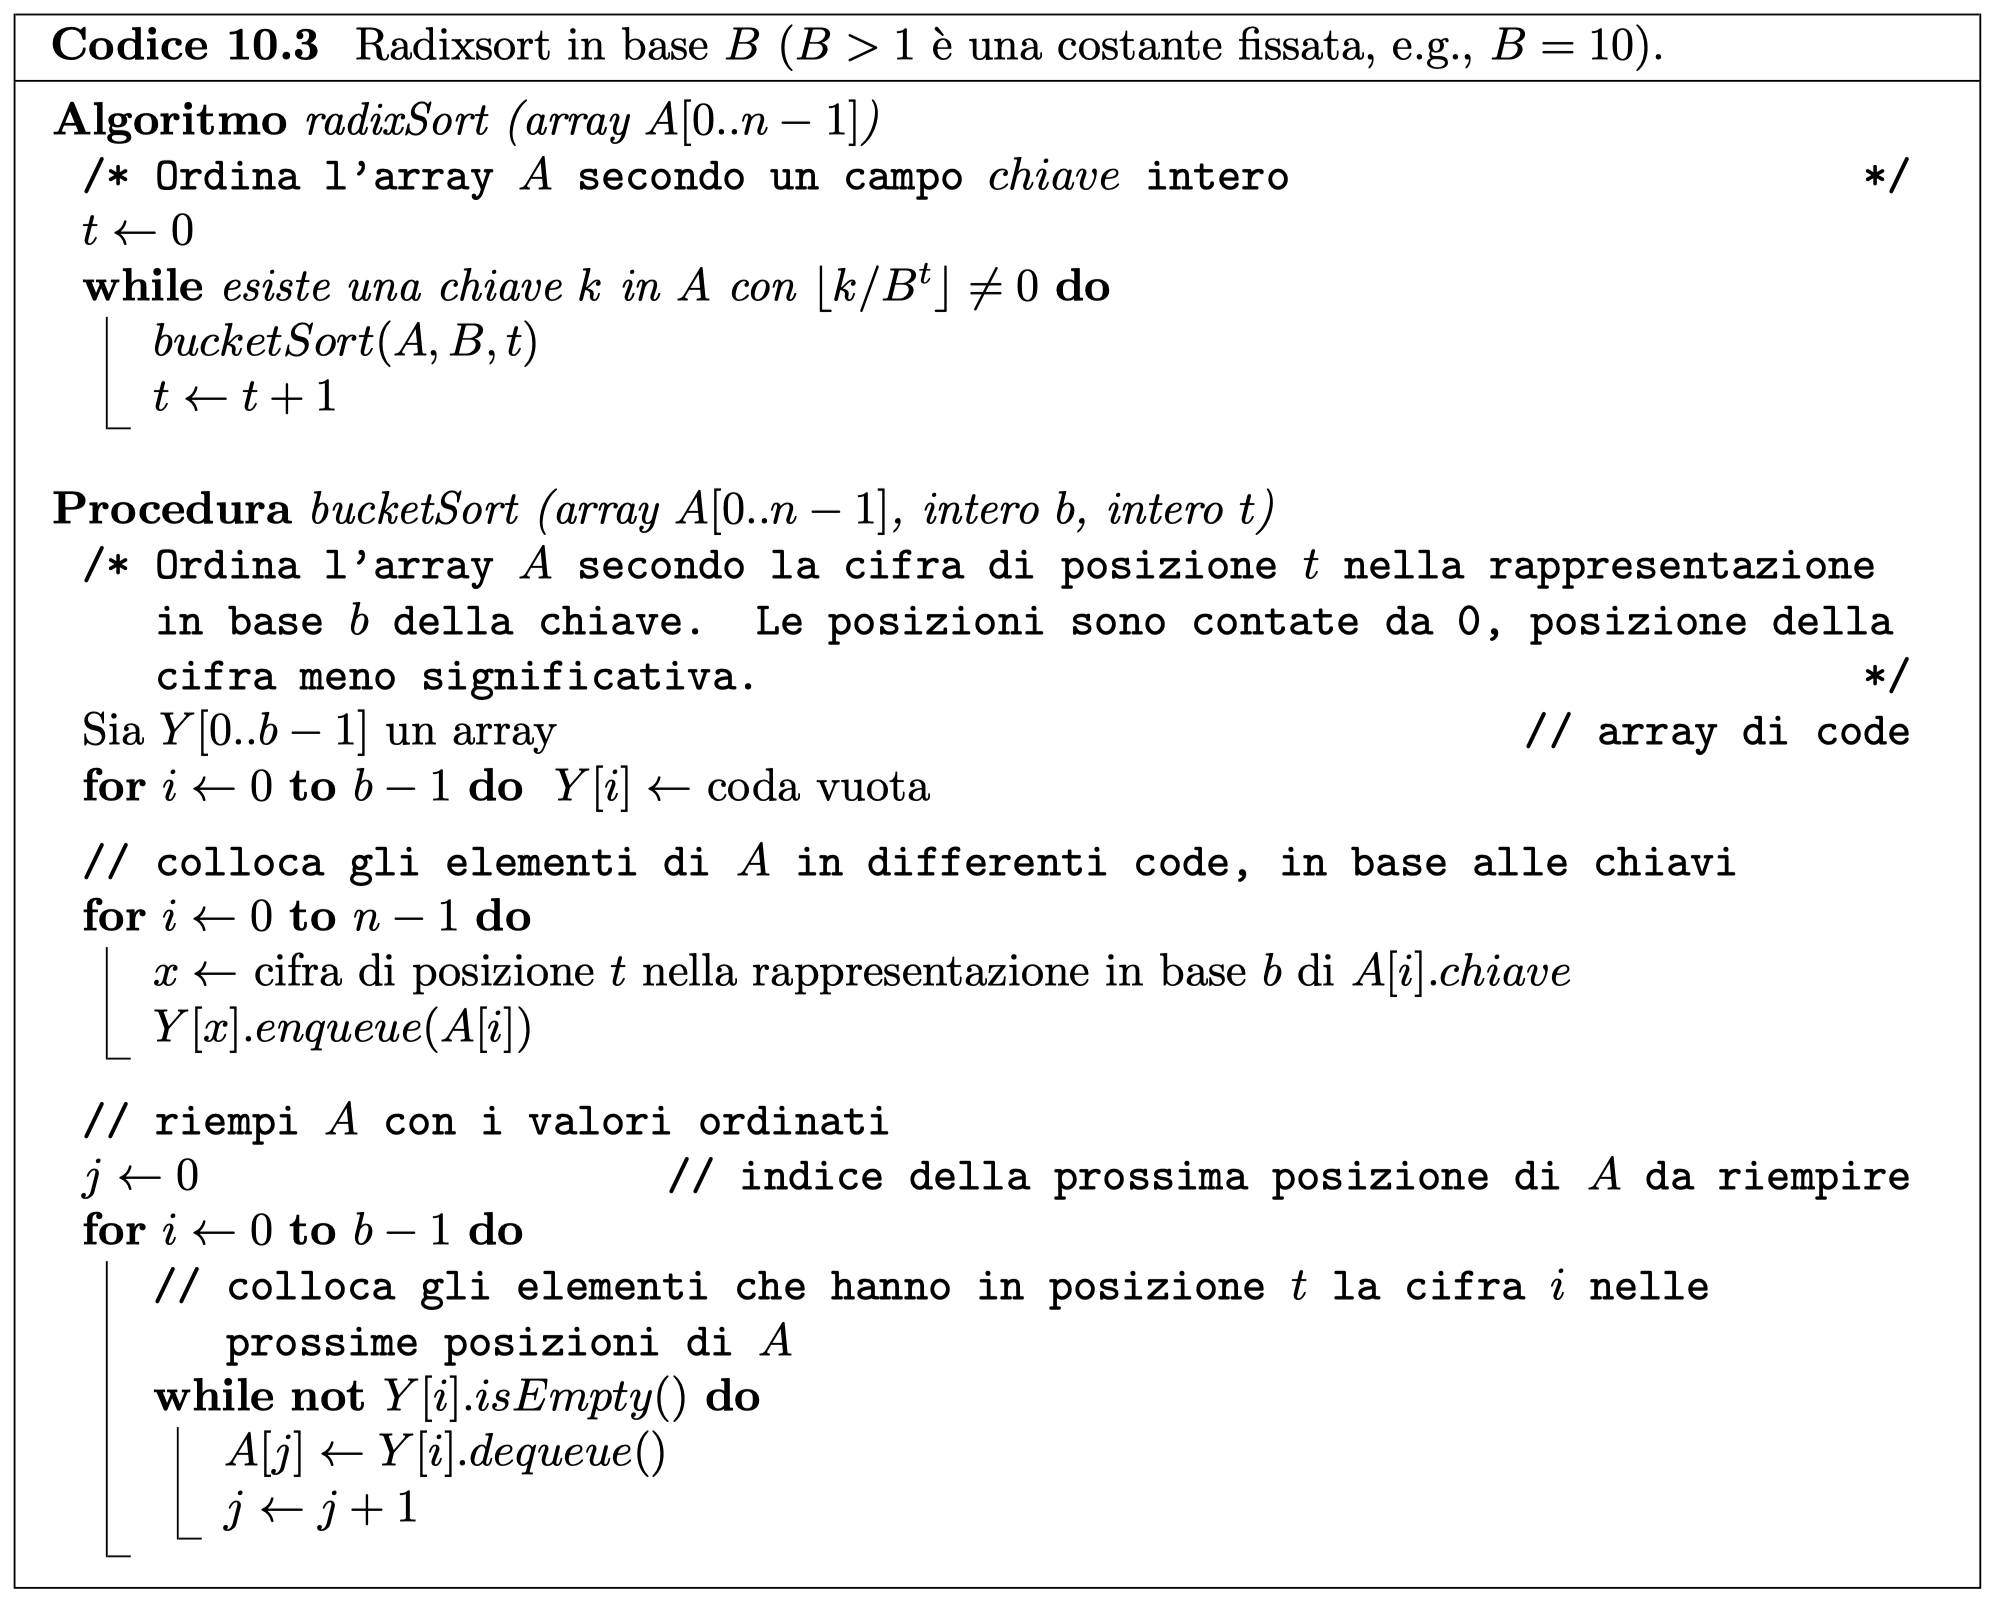
\includegraphics[width=\textwidth]{radixSort.png}
\end{figure}
\clearpage
